\documentclass[a4paper,11pt,twoside]{article}
\usepackage[T1]{fontenc}
\usepackage[utf8]{inputenc}
\usepackage{ngerman, eucal, mathrsfs, amsfonts, bbm, amsmath, amssymb, stmaryrd,graphicx, array, geometry, listings, color, ulem, epstopdf}
\geometry{left=25mm, right=15mm, bottom=25mm}
\setlength{\parindent}{0em} 
\setlength{\headheight}{0em} 
\title{Theoretische Grundlagen der Informatik II\\ Blatt 7}
\author{Markus Vieth \and Marvin Becker}
\date{\today}
\definecolor{comment_green}{rgb}{0, 0.5, 0}
\newcommand{\green}[1]{\textcolor{comment_green}{#1}}
\newcommand{\korr}[2]{\sout{#1} \textcolor{red}{\underline{#2}}}
\newcommand{\red}[1]{\textcolor{red}{#1}}

\lstset{literate=%
	{Ö}{{\"O}}1
	{Ä}{{\"A}}1
	{Ü}{{\"U}}1
	{ß}{{\ss}}2
	{ü}{{\"u}}1
	{ä}{{\"a}}1
	{ö}{{\"o}}1
	{pi}{{$\Pi$}}1
}

\begin{document}

\maketitle
\cleardoublepage
\pagestyle{myheadings}
\markboth{Markus Vieth, Marvin Becker}{Markus Vieth, Marvin Becker}

\section*{Aufgabe 1}
\subsection*{a)}
Man startet mit einem Graphen \korr{$G=/V,E)$}{$G=(V,E)$}, einem Wert \textrm{bestsofar} = $\infty$, dem Startknoten s, einer Queue S und dem Teilproblem $P_0 = (s,{s},s)$. Das Tupel ist wie folgt zu lesen : (Startknoten, Menge der Knoten zwischen Star- und Endknoten inklusive dieser, Endknoten).
Zu beginn wird das Teilproblem $P_0$ der Queue hinzugefügt.\\
In jedem Schritt des Algorithmus, wird ein Teilproblem aus der Queue genommen. Dieses Teilproblem $(a, W, b)$ wird mit einer Kante $(b, x)\in E $ mit $x\in V\setminus W$ und erhalten so ein Teilproblem $(a, W \cup {x}, x)$. Dies wird für jede Kante von $b$ wiederholt. Man erhält so die Teilprobleme $P_i$ mit $i\in {1,\ldots,n}$.
//Für jedes Teilproblem $P_i$ wird wie folgt vorgegangen.
\\Ist nun $W \cup {x} = V$, so wird die Länge des Pfades berechnet. Ist diese Länge kleiner als das bisherige \textrm{bestsofar}, dann wird \textrm{bestsofar} auf die Länge dieses Pfades gesetzt und der Pfad selbst ist die bisher beste Lösung.
\\Ist der Pfad noch nicht komplett, so wird die untere Schranke $c(W \cup {x})+c(a)+c(x)+c(T)$\footnote{siehe Vorlesung 04 Folie 11} berechnet. Ist diese kleiner, als das bisherige \textrm{bestsofar}, so wird das neue Teilproblem $P_i$ der Queue S hinzugefügt.\\
Diese Schritte werden solange wiederholt, wie sich Elemente in der Queue S befinden.\\
\korr{Irgendetwas}{Unwichtig 2/3 Punkte}
\subsection*{b)}
\begin{figure}[h]
	\hspace{-60pt}
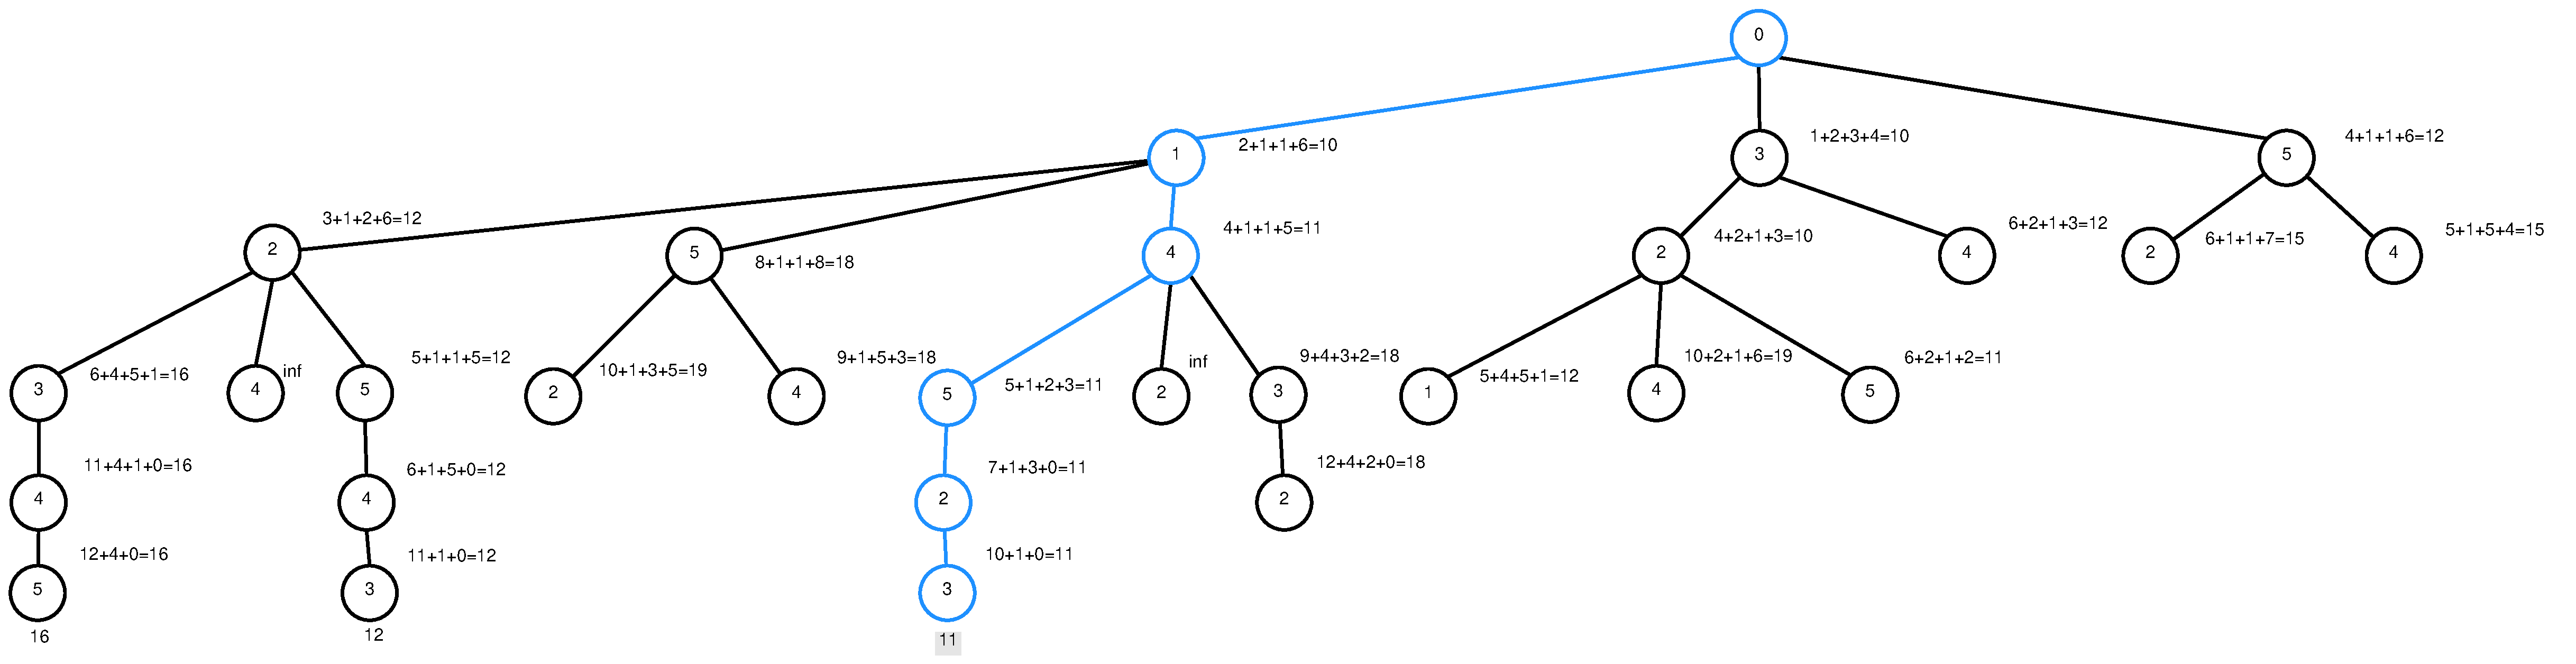
\includegraphics[width=1.2\linewidth]{Baum}
\caption{Diagramm zu Aufgabe 1}
\label{fig:Baum}
\end{figure}
Die Reihenfolge der Summanden entspricht jener aus der Formel aus Aufgabe 1 a).
\subsection*{c)}
Wie in 1b) ersichtlich, ist die kürzeste Tour $(0,1,4,5,2,3,0)$ mit den Kosten $11$.
\section*{Aufgabe 2}
\begin{tabular}{|c|c|c|c|c|c|c|c|c|c|c|c|c|}
	\hline i &  &  &  &  &  &  &  &  &  &  &  &  \\ 
	\hline 4 & 0 & 0 & 0 & 50 & 50 & 50 & 50 & 90 & 90 & 90 & 90 &  \\ 
	\hline 3 & 0 & 0 & 0 & 0 & 40 & 40 & 40 & 40 & 40 & 50 & 70 &  \\ 
	\hline 2 & 0 & 0 & 0 & 0 & 40 & 40 & 40 & 40 & 40 & 50 & 50 &  \\ 
	\hline 1 & 0 & 0 & 0 & 0 & 0 & 10 & 10 & 10 & 10 & 10 & 10 &  \\ 
	\hline 0 & 0 & 0 & 0 & 0 & 0 & 0 & 0 & 0 & 0 & 0 & 0 &  \\ 
	\hline  & 0 & 1 & 2 & 3 & 4 & 5 & 6 & 7 & 8 & 9 & 10 & W \\ 
	\hline 
	\end{tabular} \\$\Rightarrow$ Wir erhalten eine optimale Lösung für \korr{$W=10$}{$W=7$} mit den Items 2 und 4.
\section*{Aufgabe 3}


Backtracking für SAT:
Der NP-Algorithmus für SAT ( hier $f(\Phi) \rightarrow {false, true}$ ) ist true, falls eine erfüllende Belegung $(x_1, x_2, \ldots, x_n)$ für $\Phi$ existiert.\\
Um eine solche Belegung zu finden wird der Backtrack-Algorithmus angewandt:\\

Wiederhole folgende Schritte bis keine Klauseln mehr vorhanden sind:\\

Wähle eine Variable $x$ aus, die in $\Phi$ vorkommt:\\
Angenommen es existiert eine erfüllende Belegung für $\Phi$ mit $x=0$\\
$x=0$:\begin{itemize}
\item Entferne alle Klauseln in denen $\overline x$ auftritt
\item Entferne alle Literale $x$ aus den übrigen Klauseln
\item Prüfe ob Klauseln ohne Literal existieren, falls ja ist die entstandene Formel nicht erfüllbar, springe zu $x=1$
\item $f(\Phi)$ sollte nun true ergeben, falls nicht dann ist $x=0$ nicht Teil der erfüllenden Belegung
\end{itemize}
$x=1$:\\
$\Rightarrow$: Änderungen aus den vorherigen Schritten werden zurückgenommen
\begin{itemize}
\item Entferne alle Klauseln in denen $x$ auftritt
\item Entferne alle Literale $\overline x$ aus den übrigen Klauseln
\item Prüfe ob Klauseln ohne Literal existieren, falls ja existiert keine erfüllende Belegung
\item $f(\Phi)$ sollte nun true ergeben, falls nicht dann existiert keine erfüllende Belegung
\end{itemize} 
\korr{}{Baumstruktur wird nicht klar 4/5}
\end{document}

